\documentclass[10pt,journal]{IEEEtran}

\usepackage{amsmath,amssymb,amsfonts,mathtools}
\usepackage{array,booktabs,multirow,tabularx,makecell}
\usepackage{graphicx}
\usepackage{cite}
\usepackage{url}
\usepackage{xcolor}
\usepackage{enumitem}
\usepackage{siunitx}
\usepackage{microtype}
\usepackage{balance}
\usepackage{tikz}
\usetikzlibrary{arrows.meta,positioning,fit,calc,shapes.geometric}
\usepackage{algorithmic}
\usepackage[hidelinks]{hyperref}
\graphicspath{{figures/}}
\sisetup{detect-all=true}

\newcommand{\NetShield}{\textsc{NetShield}}
\newcommand{\argmax}{\operatorname*{arg\,max}}
\newcommand{\Lnone}{\textsc{L-None}}
\newcommand{\Lalert}{\textsc{L-Alert}}
\newcommand{\Lsummary}{\textsc{L-Summary}}
\newcommand{\Mnone}{\textsc{M-None}}
\newcommand{\Malert}{\textsc{M-Alert}}
\newcommand{\Msummary}{\textsc{M-Summary}}
\newcommand{\Hnone}{\textsc{H-None}}
\newcommand{\Halert}{\textsc{H-Alert}}
\newcommand{\Hsummary}{\textsc{H-Summary}}
\newcommand{\Hfull}{\textsc{H-Full}}

\begin{document}

\title{\NetShield: Shared-Bottleneck Evidence Scheduling for Multi-Probe IoT Edge Intrusion Detection}

\author{Nuonan~Ouyang,~\IEEEmembership{Member,~IEEE,}
        Adrian~Shatte,
        Zhigang~Lu,
        Chao~Chen,~\IEEEmembership{Member,~IEEE},
        and~Wei~Xiang,~\IEEEmembership{Senior~Member,~IEEE}%
\thanks{\textit{(Corresponding author: Nuonan Ouyang.)}}%
\thanks{N. Ouyang and A. Shatte are with the College of Science and Engineering, James Cook University, Bebegu Yumba Campus, Townsville, QLD, Australia (e-mail: nuonan.ouyang@my.jcu.edu.au; adrian.shatte@jcu.edu.au; ORCID: 0009-0004-7124-8940; 0000-0002-6225-9697).}%
\thanks{Z. Lu is with the School of Computer, Data and Mathematical Sciences, Western Sydney University, Penrith (Kingswood) Campus, Kingswood, NSW, Australia (e-mail: z.lu@westernsydney.edu.au; ORCID: 0000-0001-5102-6217).}%
\thanks{C. Chen is with the College of Business and Law, RMIT University, Melbourne, VIC 3000, Australia (e-mail: chao.chen@rmit.edu.au; ORCID: 0000-0003-1355-3870).}%
\thanks{W. Xiang is with the Australian Centre for AI in Medical Innovation and the Cisco--La Trobe Centre for AI and Internet of Things, La Trobe University, Melbourne, VIC, Australia (e-mail: w.xiang@latrobe.edu.au; ORCID: 0000-0002-0608-065X).}%
}

\markboth{IEEE Transactions on Networking,~Vol.~XX, No.~XX, Month~2026}%
{Ouyang \MakeLowercase{\textit{et al.}}: Shared-Bottleneck Evidence Scheduling for Multi-Probe IoT Edge IDS}

\maketitle

\begin{abstract}
Multi-probe intrusion detection at the network edge couples classification with a network-control problem: the evidence produced by concurrent decisions must traverse a common, finite service plane. If each probe chooses evidence independently, the aggregate request can exceed the shared service even when every local choice appears reasonable, creating backlog and stale evidence. This paper presents \NetShield, a runtime evidence scheduler that separates three functions: per-probe detector/evidence selection, joint pre-admission against the common bottleneck, and optional feasibility shielding. All six evaluated methods use the same capped transport service; what differs is whether the action tuple is reconciled with that shared constraint before new evidence enters the queues. The frozen action lattice contains ten detector--evidence choices spanning light, medium, and heavy local inference plus a heavy full-evidence core path.

We evaluate fixed-local, fixed-summary, fixed-full, an independent queue-aware selector (the frozen campaign label is independent-DPP), centrally pre-admitted selection (central-DPP), and its shielded counterpart on a heterogeneous Raspberry Pi~5/4B/3B+ testbed over Wi-Fi. The formal campaign contains 12 sessions, three shared-capacity regimes, 216 method--capacity arms, 648 device-runs, and 58,320 measured probe-windows. Fixed-full attains device-run macro timely F1 0.9332 but FPR 0.2845, delivers only 0.667 of generated payload over the complete 95-window runs, and reaches 7.92~MiB maximum backlog. The independent queue-aware policy restores F1/FPR to 1.0000/0.0000 and limits maximum backlog to 0.08~MiB; in aggregate measured-window accounting it generates 14.1\% more application payload than the centrally admitted policies. Central and shielded DPP both obtain F1/FPR 1.0000/0.0000 with zero observed maximum backlog and full payload delivery. Across all 9,720 measured windows per method, central and shielded DPP select identical actions; their E2E difference is not significant after Holm correction. Shielded DPP is non-inferior to fixed-summary in timely F1 at the prespecified $-0.02$ margin (difference 0.000, 95\% CI [0,0], $n=12$ sessions). The results isolate a mechanism hierarchy: queue-aware finite-action selection removes most backlog created by unreconciled fixed-full evidence generation, shared pre-admission further reduces aggregate demand and eliminates the residual queue, and the shield is non-interfering under the evaluated already-feasible central operating envelope.
\end{abstract}

\begin{IEEEkeywords}
Internet of Things, intrusion detection, edge computing, shared-link admission, drift-plus-penalty, queue-aware scheduling, feasibility shielding, Raspberry Pi.
\end{IEEEkeywords}

\section{Introduction}
Internet-of-Things (IoT) security monitoring increasingly moves inference and response toward gateways and edge nodes. This reduces cloud dependence and can shorten the path from traffic observation to action, but it also exposes a networking problem that is largely invisible in offline classifier benchmarks. A distributed IDS does not only output a label: it may retain a decision locally, transmit an alert or summary, or upload a richer feature representation for core-side processing. Those evidence paths create different byte demands and completion times, and multiple probes may request them simultaneously over the same wireless service.

This coupling matters because a method can be locally accurate and still be operationally poor. If probes choose evidence independently without reconciling simultaneous requests, aggregate generated demand can exceed the common bottleneck. The immediate decision may still execute, yet bytes accumulate in evidence queues and become progressively older. For a security service, stale evidence is qualitatively different from timely evidence: a correct result that arrives after its response horizon can no longer support the same operational claim.

The problem is also heterogeneous. A Raspberry Pi~5, Raspberry Pi~4B, and Raspberry Pi~3B+ exhibit different inference timings, but they can still compete for one common edge path. The controller must therefore retain per-probe compute and queue state while enforcing a network-wide constraint. This is different from conventional IDS model selection, where each device is usually scored independently, and from classical offloading, where the traffic demand is often treated as exogenous. Here the scheduling action itself determines how many evidence bytes enter the network queue.

We study this problem through \NetShield. The design separates three functions that are easy to conflate. First, a selector ranks a frozen set of detector/evidence actions. Second, a \emph{pre-admission} layer can reconcile simultaneous requested actions with the common bottleneck before their payload is generated. Third, a feasibility shield can remove locally unsafe actions from the candidate set. The physical service plane is common to all methods and is always capacity limited; uncoordinated baselines are allowed to \emph{request and enqueue} more evidence than that service can drain. This decomposition lets us ask which gains come from local queue awareness, which come from preventing aggregate over-generation, and whether adding the shield perturbs an already-feasible central policy.

The empirical claims in this paper use only the paper-eligible S01--S12 campaign and the frozen REV2 session-level analysis. Pilot sessions are excluded from the formal statistics, and the 36 session--capacity cells are used only for descriptive capacity interaction rather than as independent inferential replicates.

We address four research questions:
\begin{itemize}[leftmargin=1.2em]
    \item \textbf{RQ1:} Can similar or strong timely detection outcomes coexist with materially different evidence-queue and delivery behavior?
    \item \textbf{RQ2:} What is gained by network-wide shared admission beyond independent queue-aware DPP at each probe?
    \item \textbf{RQ3:} Under the evaluated operating envelope, what empirical cost or behavioral perturbation is introduced by adding the feasibility shield to central DPP?
    \item \textbf{RQ4:} Are the conclusions robust to heterogeneous Pi hardware, independently seeded sessions, and low/mid/high shared-capacity regimes under a session-level inferential analysis?
\end{itemize}

The paper makes four contributions.
\begin{enumerate}[leftmargin=1.4em]
    \item \textbf{A two-layer shared-bottleneck formulation for IDS evidence scheduling.} We distinguish \emph{action pre-admission} (which controls how many bytes are generated) from the common transport service (which drains all method queues under the same per-window cap). This prevents an important semantic ambiguity between admission and service.
    \item \textbf{A mechanism-isolating policy hierarchy with a finite discrete controller.} Six methods separate static evidence generation, independent DPP, joint capacity-constrained pre-admission, and feasibility shielding. We give the per-window controller, a finite-termination argument for monotone degradation, and the capacity/utility explanation for the observed low/mid/high action mix.
    \item \textbf{A real heterogeneous multi-probe campaign.} The evaluation uses three physical Raspberry Pi generations over Wi-Fi, 12 formal sessions, 216 arms, 648 device-runs, and 58,320 measured windows.
    \item \textbf{A corrected, frozen statistical/provenance workflow.} The independent inferential unit is the session ($n=12$), exact $2^{12}$ sign-flip tests are used, confidence intervals resample sessions as clusters, Holm correction is applied within metric families, and every manuscript number is traceable to a frozen artifact.
\end{enumerate}

\paragraph{Scope of the control claim.} The networking contribution is the separation of endogenous evidence generation, common queue service, and pre-admission over a finite action lattice. The paper does not claim a new intrusion classifier, a globally optimal joint scheduler, or a formal Lyapunov-optimal implementation of the DPP-labelled selector. These boundaries are deliberate and match the frozen rc4 execution semantics.

The headline observation is that fixed-full is not a weak-classifier baseline; it is a network-overdemand baseline. It reaches macro F1 0.9332 while building 7.92~MiB of backlog. Independent DPP largely removes that backlog and obtains timely F1 1.0000; central admission then removes the residual queue and reduces generated payload by reconciling simultaneous probe requests against the common budget. The shielded and unshielded central policies make exactly the same measured-window decisions, which is evidence of \emph{non-interference} under the tested envelope rather than evidence that shielding outperforms central DPP.

\section{Related Work}
\subsection{Lightweight IoT Intrusion Detection}
IoT intrusion-detection research has produced compact anomaly detectors, device fingerprints, and online detection pipelines for constrained hardware. Representative systems include SVELTE, IoT Sentinel, N-BaIoT, and Kitsune~\cite{raza2013svelte,miettinen2017iotsentinel,meidan2018nbaiot,mirsky2018kitsune}, together with more recent compact and graph-aware IDS designs~\cite{wang2024hyperdetect,jiang2024graph,du2024fewshot}. This literature primarily asks how to obtain useful prediction quality within a device envelope. \NetShield{} addresses a complementary runtime question: once detector and evidence choices are available, which choice can be sustained jointly across probes sharing a bottleneck?

The distinction is operationally important. Two policies may use the same frozen model family and achieve the same window-level classification outcome while imposing different network demand. Conversely, a high-richness path can lose \emph{timely} detection quality when backlog prevents evidence completion inside the response horizon. Prediction metrics are therefore necessary but insufficient for a multi-probe edge IDS.

\subsection{Edge Offloading and Communication--Computation Co-Design}
Mobile and edge computing have long studied task placement under latency, bandwidth, and energy constraints~\cite{mao2017mec,mach2017mec,chen2016offloading,mao2016dynamic}. Our setting shares the need for link-aware control, but evidence scheduling makes the traffic demand endogenous. Selecting \Hfull{} creates 131,072 application bytes, whereas a local no-evidence action creates none. The scheduler is therefore choosing both the workload and how a common service budget is used to carry that workload.

\subsection{Shared Bottlenecks, Fair Service, and Admission}
Classical fair-queueing and generalized processor-sharing work asks how a bottleneck should serve packets that have already entered competing queues~\cite{demers1989fair,parekh1993gps}. That transport problem remains present in our testbed, but it is only one layer of the IDS problem. Here the controller also decides whether a probe generates 0, 256, 4--16~KiB, or 128~KiB of new application evidence in the first place. \NetShield{} therefore separates \emph{pre-admission of a discrete evidence action tuple} from \emph{shared service of the resulting queues}. Fixed-full and independent DPP can over-generate relative to the common cap even though their queued bytes are still drained by the same capped service plane.

\subsection{Queue-Aware Network Control}
Queue-aware scheduling and Lyapunov drift-plus-penalty (DPP) provide a natural foundation for balancing instantaneous utility against queue growth~\cite{tassiulas1992stability,neely2010stochastic}. The frozen campaign retains the historical method labels independent-DPP, central-DPP, and shielded-DPP, but the deployed selector is a finite-action, queue-penalized DPP-style score rather than a claimed implementation of full Lyapunov drift minimization. We therefore make no stochastic-optimality or $O(1/V)$ theorem claim for the deployed selector. The experiment instead isolates the systems question: what changes when the same per-probe queue-aware request is reconciled against a common bottleneck before evidence generation?

\subsection{Runtime Shielding and Safe Control}
Constrained control, safe reinforcement learning, runtime shielding, and predictive safety filters separate policy optimization from hard enforcement~\cite{achiam2017cpo,garcia2015safe,alshiekh2018shielding,wabersich2021filter}. We use the same architectural principle: the shield defines an admissible action set, while the selector ranks only actions available inside that set. Importantly, our formal campaign does not manufacture unsafe episodes solely to force shield intervention. Consequently, the empirical shield claim is intentionally narrow: when central DPP remained feasible, adding the shield caused zero action changes over 9,720 measured windows.

\subsection{Federated and Collaborative IDS}
Federated IDS coordinates model training across sites while reducing raw-data exchange~\cite{mcmahan2017fedavg,nguyen2021fliot,li2021deepfed}. That problem is distinct from runtime evidence transport. \NetShield{} does not claim a new federated optimizer or a measured cross-probe correlation gain. It controls the evidence path that would support such higher-level collaboration, with the present evaluation limited to detector/evidence scheduling, shared-link service, queue behavior, and timely outcomes.

\subsection{Relation to Our Prior Runtime-Assurance SoK}
Our prior ACISP 2026 Systematization of Knowledge (SoK) surveyed telemetry-aware, always-on on-device IDS and proposed TQS-IDS as a corpus-grounded interface template for composing telemetry, actuation, and runtime constraints~\cite{ouyang2026sok}. That publication explicitly did not implement or empirically validate TQS-IDS. The present paper is not a journal extension of an earlier NetShield experiment: it formulates the distinct networking problem of discrete evidence generation over a shared bottleneck, introduces DPP-based per-probe selection plus joint pre-admission, and evaluates the resulting mechanism hierarchy in the S01--S12 Raspberry-Pi campaign. None of the NetShield hardware results, shared-bottleneck statistics, or session-level contrasts reported here appeared in the SoK.

\section{System Model and Design}
\subsection{Two-Layer Shared-Bottleneck Model}
Consider $N$ probes indexed by $i$ and a local edge core. Time is divided into scheduling windows $t$. Probe $i$ observes a frozen feature vector $x_i(t)$ and maintains an evidence queue $Q_i(t)$. Each policy first produces a \emph{requested} action $r_i(t)$; a centrally coordinated method may replace it with an \emph{admitted} action $a_i(t)$ before the new payload is generated. Let $b(a)$ be the application bytes generated by action $a$.

All six methods then use the same transport service plane. If $g_i(t)$ is the number of queued application bytes drained for probe $i$ during window $t$, the shared service satisfies
\begin{equation}
    g_i(t)\ge 0,\qquad \sum_{i=1}^{N} g_i(t)\le C(t),
    \label{eq:sharedcap}
\end{equation}
where $C(t)$ is the configured per-window application-service budget. The queue evolves as
\begin{equation}
    Q_i(t+1)=\left[Q_i(t)+b(a_i(t))-g_i(t)\right]^+.
    \label{eq:queue}
\end{equation}
This distinction is central to the experiment. For A--D, $a_i(t)=r_i(t)$: the method does not jointly reduce simultaneous requests before bytes enter the queues, so $\sum_i b(a_i(t))$ may exceed $C(t)$. The shared service in~\eqref{eq:sharedcap} still limits how quickly those queues drain. For E/F, the requested tuple is reconciled with the shared cap before generation, so the controller seeks an admitted tuple whose new-byte demand is feasible. Figure~\ref{fig:architecture} shows the resulting pipeline.

\begin{figure*}[t]
\centering
\resizebox{0.97\textwidth}{!}{%
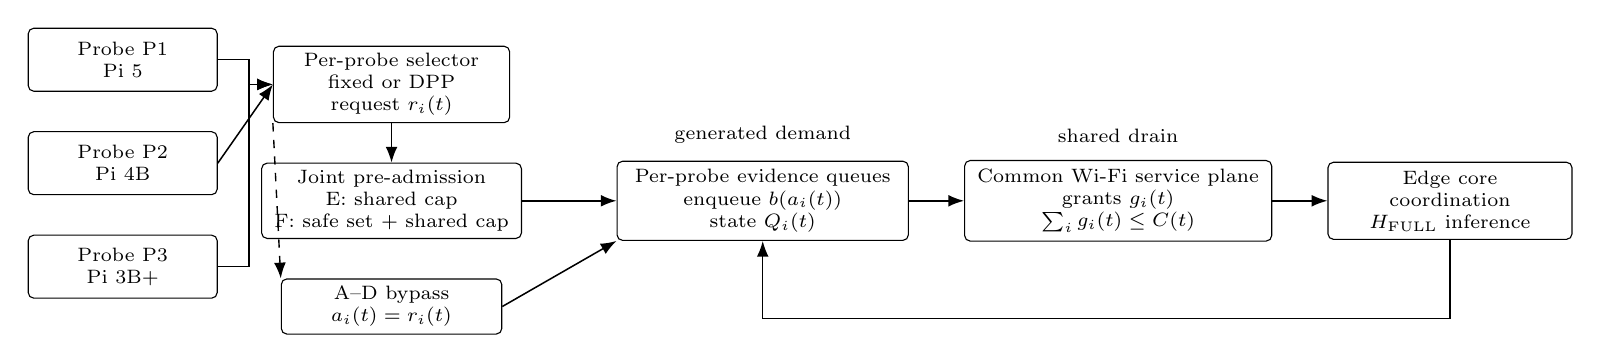
\begin{tikzpicture}[
    font=\scriptsize,
    node distance=5mm and 7mm,
    box/.style={draw, rounded corners=2pt, minimum height=8mm, align=center, inner sep=3pt},
    smallbox/.style={draw, rounded corners=2pt, minimum height=7mm, align=center, inner sep=2.5pt},
    arr/.style={-{Latex[length=2mm]}, line width=0.55pt},
    dashedarr/.style={-{Latex[length=2mm]}, dashed, line width=0.5pt}
]
\node[box, minimum width=24mm] (p1) {Probe P1\\Pi 5};
\node[box, minimum width=24mm, below=of p1] (p2) {Probe P2\\Pi 4B};
\node[box, minimum width=24mm, below=of p2] (p3) {Probe P3\\Pi 3B+};

\node[smallbox, minimum width=30mm, right=of p2, yshift=10mm] (sel) {Per-probe selector\\fixed or DPP\\request $r_i(t)$};
\node[smallbox, minimum width=33mm, below=of sel] (preadm) {Joint pre-admission\\E: shared cap\\F: safe set + shared cap};
\node[smallbox, minimum width=28mm, below=of preadm] (raw) {A--D bypass\\$a_i(t)=r_i(t)$};

\node[box, minimum width=37mm, right=12mm of preadm] (queues) {Per-probe evidence queues\\enqueue $b(a_i(t))$\\state $Q_i(t)$};
\node[box, minimum width=39mm, right=of queues] (service) {Common Wi-Fi service plane\\grants $g_i(t)$\\$\sum_i g_i(t)\le C(t)$};
\node[box, minimum width=31mm, right=of service] (core) {Edge core\\coordination\\$H_{\mathrm{FULL}}$ inference};

\draw[arr] (p1.east) -- ++(4mm,0) |- (sel.west);
\draw[arr] (p2.east) -- (sel.west);
\draw[arr] (p3.east) -- ++(4mm,0) |- (sel.west);
\draw[arr] (sel) -- (preadm);
\draw[dashedarr] (sel.south west) -- (raw.north west);
\draw[arr] (preadm.east) -- (queues.west);
\draw[arr] (raw.east) -- (queues.south west);
\draw[arr] (queues) -- (service);
\draw[arr] (service) -- (core);
\draw[arr] (core.south) |- ++(-40mm,-10mm) -| (queues.south);

\node[align=center, above=1mm of queues] {generated demand};
\node[align=center, above=1mm of service] {shared drain};
\end{tikzpicture}%
}
\caption{\NetShield{} execution semantics. The shared transport service and queues exist for every method. A--D differ from E/F because their requested actions are not jointly pre-admitted before new evidence is generated; E/F reconcile the requested tuple with the common budget, while F additionally filters the candidate set through the feasibility shield.}
\label{fig:architecture}
\end{figure*}

\subsection{Frozen Ten-Action Lattice and Utility}
The deployed action set contains ten joint detector/evidence choices spanning light (L), medium (M), and heavy (H) detector tiers. Table~\ref{tab:actions} lists the frozen application payloads and scheduling utilities. Detector strength and evidence richness are only partially coupled: all three local tiers can retain no network evidence, emit a 256-byte alert, or emit a tier-specific summary; the heavy tier additionally supports the 131,072-byte full-evidence core path.

\begin{table}[t]
\centering
\caption{Frozen action lattice. Utility is a pre-campaign scheduling score, not a universal performance ranking.}
\label{tab:actions}
\scriptsize
\setlength{\tabcolsep}{3.0pt}
\begin{tabular}{@{}llllrr@{}}
\toprule
Action & Detector & Exec. & Evidence & Payload (B) & Utility\\
\midrule
\Lnone{}    & light  & local & none    & 0       & 0.758501\\
\Lalert{}   & light  & local & alert   & 256     & 0.825168\\
\Lsummary{} & light  & local & summary & 4,096   & 0.891835\\
\Mnone{}    & medium & local & none    & 0       & 0.766968\\
\Malert{}   & medium & local & alert   & 256     & 0.833635\\
\Msummary{} & medium & local & summary & 8,192   & 0.900302\\
\Hnone{}    & heavy  & local & none    & 0       & 0.768378\\
\Halert{}   & heavy  & local & alert   & 256     & 0.835044\\
\Hsummary{} & heavy  & local & summary & 16,384  & 0.901711\\
\Hfull{}    & heavy  & core  & full    & 131,072 & 0.968378\\
\bottomrule
\end{tabular}
\end{table}

The utility is frozen from validation balanced accuracy and evidence richness:
\begin{equation}
  u(a)=0.8\,v_{\mathrm{det}}(d(a))+0.2\,v_{\mathrm{ev}}(e(a)),
  \label{eq:utility}
\end{equation}
where $v_{\mathrm{ev}}\in\{0,1/3,2/3,1\}$ for none, alert, summary, and full evidence. The detector terms are pre-campaign validation balanced accuracies; the resulting action utilities in Table~\ref{tab:actions} are frozen before S01--S12. These weights are an explicit design choice rather than an optimization claim.

\subsection{Queue-Aware Selection and Joint Pre-Admission}
For the adaptive methods, each probe ranks the finite candidate set using the queue-penalized score implemented by the frozen campaign,
\begin{equation}
\begin{aligned}
  \psi_i(a,t)&=v_{\mathrm{DPP}}u(a)-\frac{Q_i(t)b(a)}{10^{6}},\\
  r_i(t)&=\argmax_{a\in\mathcal A_i(t)}\psi_i(a,t).
\end{aligned}
  \label{eq:dpp}
\end{equation}
where $v_{\mathrm{DPP}}=1.0$ in all three formal low/mid/high campaign configurations. We retain the campaign's DPP method labels for provenance, but Eq.~\eqref{eq:dpp} is used here as the implemented queue-aware selection score; we do not claim that the deployed code solves a full stochastic Lyapunov drift minimization. Independent-DPP (D) stops at this step: each probe reacts to its own queue but does not coordinate the simultaneous evidence it generates with the other probes.

Central-DPP (E) adds deterministic joint pre-admission. Starting from the requested tuple $\mathbf r(t)$, the coordinator applies the frozen monotone degradation and tie-breaking rules until the admitted tuple $\mathbf a(t)$ satisfies
\begin{equation}
       \sum_{i=1}^{N} b(a_i(t))\le C(t).
 \label{eq:joint}
\end{equation}
The stage is therefore a finite feasibility/reconciliation procedure, not a claim that the implementation globally solves a $K^N$ joint argmax in every state. The common transport service in~\eqref{eq:sharedcap} executes afterward and drains every method's queues under the same shared budget.

The frozen utility ordering together with the deterministic degradation rule explains the observed capacity gradient when E/F queues are empty. At low capacity, three \Hsummary{} actions use 49,152~B and have aggregate utility 2.705133, exceeding one \Hfull{} plus two \Hnone{} actions (131,072~B, utility 2.505134). At mid capacity, one \Hfull{} plus two \Hsummary{} actions use 163,840~B and have aggregate utility 2.771800, exceeding two \Hfull{} plus one \Hnone{} action (262,144~B, utility 2.705134). At high capacity, three \Hfull{} actions fit exactly and have aggregate utility 2.905134. Thus the measured low/mid/high action mix is consistent with the frozen discrete utility--payload ordering and pre-admission rule, rather than being an arbitrary capacity label.

\subsection{Feasibility Shield}
Shielded DPP (F) changes the candidate set, not the DPP objective. Let the frozen feasibility predicates be $h_k(s_i(t),a)\le0$, where $s_i(t)$ contains the observed/predicted local and network state. The safe set is
\begin{equation}
  \mathcal A_i^{\mathrm{safe}}(t)
  =\{a\in\mathcal A: h_k(s_i(t),a)\le0\ \forall k\}.
  \label{eq:safeset}
\end{equation}
F replaces $\mathcal A$ by $\mathcal A_i^{\mathrm{safe}}(t)$ in~\eqref{eq:joint}; E does not. The predicates encode the configured operating envelope, while the joint capacity constraint remains explicit. Importantly, satisfying the configured predictor boundary is not an unconditional guarantee on realized Wi-Fi completion time. Section~VI reports one F deadline miss caused by an isolated transport RTT spike despite zero queue backlog.

\textbf{Proposition 1 (nonempty and finite admission).}
Assume each probe's candidate set contains a zero-payload local fallback and that infeasible requests are monotonically degraded along the finite action order. Then a feasible joint action exists for any $C(t)\ge0$, and admission terminates after at most $N(K-1)$ strict degradations for $K$ action levels.

\emph{Proof.} The all-zero-payload tuple is feasible for any nonnegative cap. Every strict degradation decreases a probe's finite action rank and never increases its payload. A probe can therefore be degraded at most $K-1$ times, so the process terminates after at most $N(K-1)$ strict steps. \hfill$\square$

This proposition is deliberately limited to configured byte feasibility. It does not imply zero deadline misses, zero packet loss, or universal queue stability under an arbitrarily misestimated physical service process.

\subsection{Per-Window Runtime Procedure}
Figure~\ref{alg:runtime} states the controller at the level used by the experiment. It highlights the separation between action generation and queue service that is otherwise easy to obscure in prose.

\begin{figure}[t]
\centering
\begin{minipage}{0.96\columnwidth}
\small
\textbf{Algorithm 1: One scheduling window}\par
\vspace{1mm}
\begin{algorithmic}[1]
\STATE Read $x_i(t)$, $Q_i(t)$ and current state for all probes
\STATE Build per-probe candidate sets (safe sets only for F)
\STATE Produce requested actions $r_i(t)$ (fixed policy or DPP ranking)
\IF{method is E or F}
  \STATE Jointly pre-admit/degrade requests under $\sum_i b(a_i)\le C(t)$
\ELSE
  \STATE Set $a_i(t)\leftarrow r_i(t)$ for every probe
\ENDIF
\STATE Enqueue the generated evidence $b(a_i(t))$
\STATE Allocate common transport grants $g_i(t)$ with $\sum_i g_i(t)\le C(t)$
\STATE Drain queues, execute local/core inference path, and timestamp completion
\STATE Log action, bytes, queue, latency, device state, and identity fields
\end{algorithmic}
\end{minipage}
\caption{Per-window runtime semantics. The common transport service applies to every method; E/F additionally control demand before queue insertion.}
\label{alg:runtime}
\end{figure}

For $K=10$ actions, local scoring requires $O(NK)$ score evaluations per window. The monotone pre-admission stage does not require exhaustive $K^N$ enumeration: because every strict degradation reduces a finite action rank, at most $N(K-1)$ degradations are needed before the zero-payload fallback is reached. This finite discrete structure keeps the control procedure lightweight in the three-probe deployment; the primary campaign nevertheless reports end-to-end behavior rather than claiming a separate microbenchmark for scheduler CPU time.

\subsection{What the Six Methods Isolate}
Table~\ref{tab:methods} summarizes the hierarchy. The critical distinction is \emph{pre-admission awareness}, not whether a method experiences the shared service: every method's queued evidence is carried by the same capped service plane. A--D can generate more new bytes than the common cap in a window; E/F prevent that aggregate over-generation before queue insertion.

\begin{table}[t]
\centering
\caption{Six frozen methods and the mechanism isolated by each comparison.}
\label{tab:methods}
\scriptsize
\setlength{\tabcolsep}{2.7pt}
\begin{tabular}{@{}clp{4.55cm}@{}}
\toprule
ID & Method & Runtime semantics\\
\midrule
A & fixed-local & Always \Hnone; zero application payload; shared service therefore has no evidence bytes to drain.\\
B & fixed-summary & Always \Hsummary; request generation is not jointly pre-admitted, but queued bytes use the common service plane.\\
C & fixed-full & Always \Hfull; deliberately over-generates at low/mid capacity and exposes structural backlog under the common service.\\
D & independent-DPP & Queue-aware per-probe selection; no joint pre-admission of simultaneous requests.\\
E & central-DPP & DPP plus joint capacity-constrained pre-admission before evidence generation.\\
F & shielded-DPP & E plus safe-action filtering before joint pre-admission.\\
\bottomrule
\end{tabular}
\end{table}

\section{Experimental Methodology}
\subsection{Physical Testbed and Frozen Workload}
The formal campaign uses three heterogeneous physical probes: P1 is a Raspberry Pi~5, P2 a Raspberry Pi~4B, and P3 a Raspberry Pi~3B+. All probe--core experiment traffic uses Wi-Fi. The local edge core hosts coordination and the core execution path for \Hfull. Before/after wireless-environment evidence and run identities are retained for the campaign so that the execution context can be audited independently of the result tables.

The workload is a frozen CICIoT2023-derived feature-vector replay rather than packet replay. Detector models, feature order, action profiles, and window plans are frozen before S01--S12. The detector pool is not presented as a new classifier benchmark: the study holds the models fixed and evaluates whether scheduling and evidence freshness preserve operationally timely decisions. The ceiling F1 values observed for several methods are therefore properties of this controlled replay, not claims of state-of-the-art open-world detection. Each device/arm contains 5 warm-up windows followed by 90 measured windows; warm-up windows are excluded from the inferential detection statistics. The released formal low/mid/high JSON configurations all set \texttt{dpp\_v}=1.0, \texttt{window\_seconds}=1.0, \texttt{windows}=95, \texttt{warmup\_windows}=5, and \texttt{deadline\_ms}=1000.0; the three files are included with the reproducibility bundle. The formal campaign therefore contains
\[
12\;\text{sessions}\times 3\;\text{capacities}\times 6\;\text{methods}=216\;\text{arms},
\]
with three device-runs per arm, giving 648 device-runs and $648\times90=58{,}320$ measured probe-windows. Each method contributes 108 device-runs and 9,720 measured windows.

\subsection{Shared-Capacity Regimes}
The controlled service budgets are shown in Table~\ref{tab:capacity}. They are application-service budgets imposed on the real Wi-Fi transport, not claims about three commercial PHY rates. The same shared service plane drains evidence queues for all six methods. E/F additionally use the budget as a \emph{pre-admission} constraint on new action payload; A--D do not. The values are aligned with the 131,072-byte \Hfull{} payload: low equals one full-payload equivalent, mid two, and high three.

\begin{table}[t]
\centering
\caption{Configured shared application-service budget per scheduling window.}
\label{tab:capacity}
\small
\begin{tabular}{@{}lrr@{}}
\toprule
Regime & Shared cap (B/window) & Full-evidence equivalents\\
\midrule
Low  & 131,072 & 1\\
Mid  & 262,144 & 2\\
High & 393,216 & 3\\
\bottomrule
\end{tabular}
\end{table}

This design makes coordination observable. Three simultaneous \Hfull{} requests total 393,216~B. They fit exactly in the high regime, exceed mid by 131,072~B, and exceed low by 262,144~B. For C/D, those excess generated bytes can enter queues and are subsequently drained by the common service. For E/F, the requested tuple is reduced before generation. The comparison therefore isolates \emph{over-generation versus pre-admission}, not two different physical links.

\subsection{Metrics}
\textbf{Timely detection.} We report timely F1 and false-positive rate (FPR). The primary method table uses unweighted means of the 108 device-runs per method. These are macro averages across physical runs, not a pooled-window micro average. For fixed-full, the macro values are F1 0.933168 and FPR 0.284536 (reported as 0.9332/0.2845); pooling its window-level confusion counts instead gives 0.933589/0.282292 (0.9336/0.2823).

\textbf{Evidence completion.} Mean E2E is the mean of per-run evidence completion times. Deadline-violation rate is computed per run and then averaged. The configured deadline is 1,000~ms.

\textbf{Queue and delivery.} MaxQ is the largest queue backlog observed across runs, reported in MiB ($2^{20}$ bytes). The table's queue-violation rate is a separate configured hard-predicate indicator; a value of zero therefore does not imply zero backlog. Delivered/generated ratios are computed from application payload bytes. The main table uses the full 95-window run so warm-up backlog drainage cannot inflate the ratio above one. The independent-DPP measured-only ratio is 1.004 because warm-up backlog drains during the measured phase; its full-run ratio is 0.998.

\textbf{Queue age.} A separate descriptive diagnostic counts windows in which the oldest queued evidence exceeds 10 windows. This is distinct from the primary queue-violation field and is used to show how structural backlog becomes stale under fixed-full.

\subsection{Statistical Analysis}
The independent inferential unit is the session ($n=12$). Within each session and method, the three capacities and three devices are pooled before forming the paired session difference: confusion matrices are summed; E2E and violation counts are pooled over windows. The 36 $(\text{session},\text{capacity})$ cells are reported descriptively but are not treated as independent replicates.

For every pairwise contrast, the frozen REV2 pipeline performs an exact two-sided sign-flip test over all $2^{12}=4{,}096$ session sign assignments. Confidence intervals use a 10,000-resample session-cluster bootstrap with seed 20260828. Holm--Bonferroni correction is applied separately inside each metric family (15 method pairs per family). The figure bootstrap uses 10,000 resamples with a separate fixed seed, 20260904. The prespecified non-inferiority comparison is shielded-DPP versus fixed-summary in timely F1 with margin $-0.02$. Generated-payload totals and action-transition counts are reported as descriptive mechanism diagnostics; they were not included in the five prespecified inferential metric families.

This session-level analysis supersedes an earlier 36-cell analysis that incorrectly treated the three capacities inside a session as independent. No raw S01--S12 data were changed during the correction.

\section{Results}
\subsection{RQ1: Detection Quality and Queue Sustainability Diverge}
Table~\ref{tab:primary} gives the primary method-level summary. A, B, D, E, and F all obtain timely F1 1.0000 and FPR 0.0000. Fixed-full (C), however, falls to F1 0.9332 and FPR 0.2845 while reaching 7.92~MiB maximum backlog. The contrast is not a classifier substitution effect: it is the consequence of a fixed 131,072-byte evidence demand that is not reconciled against the common low/mid capacity.

\begin{table*}[t]
\centering
\caption{Per-method performance across the 12 formal sessions (216 arms, 648 device-runs, 58,320 measured windows). Timely-F1/FPR are unweighted means across the 108 device-runs per method (macro-average; the pooled-window micro-average for C is F1 $=$ 0.9336, FPR $=$ 0.2823). E2E is the mean of per-run evidence completion times; violation rates are per measured window, averaged across runs. Deliv/Gen is the delivered/generated payload-byte ratio over all 95 windows including warm-up; A uploads no application payload. MaxQ is in MiB.}
\label{tab:primary}
\scriptsize
\setlength{\tabcolsep}{3.1pt}
\begin{tabular}{@{}lrrrrrrrr@{}}
\toprule
Method & Runs & Timely-F1 & FPR & E2E (ms) & Deadline-viol. & Queue-viol. & Deliv/Gen & MaxQ (MiB)\\
\midrule
fixed-local (A) & 108 & 1.0000 & 0.0000 & 672.9 & 0.000000 & 0.000000 & n/a & 0.00\\
fixed-summary (B) & 108 & 1.0000 & 0.0000 & 673.1 & 0.000000 & 0.000000 & 1.000 & 0.00\\
fixed-full (C) & 108 & 0.9332 & 0.2845 & 693.2 & 0.000000 & 0.000000 & 0.667 & 7.92\\
independent-DPP (D) & 108 & 1.0000 & 0.0000 & 660.1 & 0.000000 & 0.000000 & 0.998 & 0.08\\
central-DPP (E) & 108 & 1.0000 & 0.0000 & 670.8 & 0.000000 & 0.000000 & 1.000 & 0.00\\
shielded-DPP (F) & 108 & 1.0000 & 0.0000 & 665.0 & 0.000103 & 0.000000 & 1.000 & 0.00\\
\bottomrule
\end{tabular}
\end{table*}

The capacity interaction in Fig.~\ref{fig:capacity} makes the mechanism visible. Using capacity-specific pooled confusion matrices for description, C has F1/FPR 0.9375/0.2797 at low, 0.8634/0.5672 at mid, and 1.0000/0.0000 at high. All other methods are 1.0000/0.0000 at all three capacities. C's oldest-evidence age diagnostic is violated in 2,916/3,240 low-capacity windows (90.0\%) and 2,376/3,240 mid-capacity windows (73.3\%), but in 0/3,240 high-capacity windows. Thus, the loss in timely detection appears exactly where the fixed-full evidence stream becomes persistently stale.

\begin{figure*}[t]
\centering

\includegraphics[width=\textwidth]{fig1_capacity_interaction.png}
\caption{Capacity--method interaction. Points are session-level means with 95\% session-bootstrap confidence intervals ($n=12$ sessions per capacity--method cell; devices pooled). Fixed-full is the only method whose timely F1/FPR degrades at low/mid capacity; E2E differences are smaller and more variable.}
\label{fig:capacity}
\end{figure*}

Session-level inference confirms the fixed-full effect. Relative to shielded-DPP, C has a timely-F1 difference of $-0.06649$ (95\% CI $[-0.07008,-0.06264]$, exact $p=0.000488$, Holm $p=0.007324$) and an FPR difference of $+0.28172$ (95\% CI $[0.26799,0.29621]$, exact $p=0.000488$, Holm $p=0.007324$). All 12 sessions place C below the other methods in timely F1, yielding the minimum two-sided exact sign-flip probability available for a 12-pair sample.

\subsection{RQ2: Shared Pre-Admission Reduces Demand Beyond Independent DPP}
Independent DPP (D) already removes almost all of C's queue problem: its maximum backlog is 87,382~B (0.08~MiB), and its timely F1/FPR are 1.0000/0.0000. This demonstrates the first benefit of queue-aware selection. But D still chooses actions independently across probes before the common service drains their queues. Across the measured windows it generates 747,307,008~B, compared with 654,704,640~B for central/shielded DPP, i.e., 14.1\% more application payload. This 14.1\% figure is descriptive aggregate accounting rather than a prespecified session-level hypothesis test. Its action trace also differs from F in 5,940 of the 9,720 measured windows. The dominant D$\rightarrow$F changes are \Hnone$\rightarrow$\Hsummary{} (2,736 windows), \Hfull$\rightarrow$\Hsummary{} (1,872), \Msummary$\rightarrow$\Hsummary{} (792), and \Hnone$\rightarrow$\Hfull{} (540), directly showing that shared admission changes the evidence mix rather than merely changing accounting after selection.

Central pre-admission changes the action mix before bytes enter the queues, while the downstream service plane remains the same. For both E and F, low capacity produces 16,384~B per probe-window (all \Hsummary), high produces 131,072~B per probe-window (all \Hfull), and mid averages 54,613.33~B per probe-window, exactly corresponding to one \Hfull{} plus two \Hsummary{} actions per three-probe scheduling window. Aggregate admitted demand therefore adapts to the shared bottleneck rather than assigning each probe an independent copy of the nominal cap.

The benefit is principally resource-side rather than latency-side. E and D have identical timely F1/FPR, and their mean-E2E difference (E$-$D) is $+10.76$~ms (95\% CI $[-6.62,31.97]$), with Holm-adjusted $p=1.0$. E therefore does not obtain a statistically supported E2E improvement over D. Instead, it removes D's residual maximum queue and lowers generated bytes while preserving timely detection.

Fixed-full provides a useful latency reference. C is 33.15~ms slower than D in session-level mean E2E (95\% CI $[19.80,48.33]$, exact $p=0.000977$, Holm $p=0.01465$) and 28.21~ms slower than F (95\% CI $[19.19,36.56]$, exact $p=0.001465$, Holm $p=0.02051$). The analysis does \emph{not} support claiming that C is significantly slower than every method; only the C--D and C--F E2E contrasts survive Holm correction.

\subsection{RQ3: Shielding Is Non-Interfering Under the Evaluated Envelope}
The most important F-versus-E result is a null action difference. Their measured-window key sets are identical and all 9,720 actions match exactly. The shield therefore never changes a central-DPP action in the formal measured windows. This should not be interpreted as evidence that the shield is unnecessary, nor as evidence that F ``beats'' E. It shows that under this campaign's already-feasible central operating envelope, the extra enforcement layer is behaviorally non-interfering.

The outcome metrics agree with that interpretation. E and F both obtain timely F1 1.0000, FPR 0.0000, MaxQ 0, and full payload delivery. Their session-level E2E difference (E$-$F) is $+5.81$~ms with 95\% CI $[-7.88,20.85]$ (exact $p=0.4902$, Holm $p=1.0$). Timely-F1 and FPR differences are exactly zero with Holm $p=1.0$.

F does record one deadline violation among 9,720 measured windows, giving the Table~\ref{tab:primary} macro violation rate of 0.000103. The event occurs in S09/high/P3/window~80: decision latency is 1,315.09~ms against the 1,000-ms deadline and evidence receipt RTT is 1,311.90~ms, while the queue is empty and neighboring windows are near 60--70~ms RTT. This isolated event is consistent with transient wireless transport jitter and demonstrates why a feasibility filter based on observed/predicted state should not be described as an unconditional zero-violation certificate.

The prespecified non-inferiority test provides an additional detection-side check. For shielded-DPP minus fixed-summary timely F1, the mean session difference is 0.000 with 95\% CI $[0,0]$; with margin $-0.02$, $n=12$ sessions, and the exact sign-flip procedure, F meets non-inferiority. The associated Holm-adjusted equality-test $p$ is 1.0; the non-inferiority conclusion follows from the margin and observed difference, not from rejecting an equality null.

\begin{table}[t]
\centering
\caption{Key frozen session-level inferential results. Differences use method A minus method B in each row. CIs are 10,000-resample session-cluster bootstrap intervals; tests are exact $2^{12}$ sign-flip; Holm correction is within each metric family.}
\label{tab:inference}
\scriptsize
\setlength{\tabcolsep}{2.8pt}
\begin{tabular}{@{}llrrr@{}}
\toprule
Metric & Contrast & Difference & 95\% CI & Holm $p$\\
\midrule
Timely F1 & C$-$F & $-0.06649$ & $[-0.07008,-0.06264]$ & 0.00732\\
FPR & C$-$F & $+0.28172$ & $[0.26799,0.29621]$ & 0.00732\\
E2E (ms) & C$-$F & $+28.21$ & $[19.19,36.56]$ & 0.02051\\
E2E (ms) & C$-$D & $+33.15$ & $[19.80,48.33]$ & 0.01465\\
E2E (ms) & E$-$F & $+5.81$ & $[-7.88,20.85]$ & 1.000\\
Timely F1 & E$-$F & $0.00000$ & $[0,0]$ & 1.000\\
\bottomrule
\end{tabular}
\end{table}

\subsection{RQ4: Session and Capacity Robustness}
The formal inference does not treat 58,320 windows as independent replications. Each of the 12 sessions contributes one paired value per method contrast after pooling its three capacities and three devices. This conservative structure matters because the capacity runs within a session share the same physical pool and experimental context.

The capacity-specific figure nevertheless shows a stable qualitative pattern: C degrades at low/mid and recovers at high; E/F adapt their evidence mix to capacity and retain zero backlog; D retains correct timely outcomes with a small residual queue. Fig.~\ref{fig:e2e} shows that E2E varies substantially by session, particularly at high capacity, which explains why many pairwise E2E differences are not significant even when their grand means differ numerically.

\begin{figure*}[t]
\centering

\includegraphics[width=\textwidth]{fig2_e2e_by_capacity.png}
\caption{Distribution of the 12 session-mean E2E values for each method, faceted by capacity. The figure emphasizes between-session variability and should be read with the session-level inferential table rather than as 36 independent replicates.}
\label{fig:e2e}
\end{figure*}

\section{Discussion}
\subsection{Queue Awareness Limits Backlog; Shared Pre-Admission Controls Generation}
The strongest evidence in the campaign is the progression from C to D to E/F. C sends the richest path unconditionally and is the only method with large persistent backlog and degraded timely detection. D introduces local queue awareness and almost eliminates backlog. E/F then solve the remaining coordination problem: their aggregate request is reconciled against the common budget, measured-window payload is 14.1\% lower than D, and the residual queue disappears without sacrificing timely F1/FPR. The data therefore attribute the large C$\rightarrow$D gain to queue awareness and support a descriptive D$\rightarrow$E/F resource-efficiency gain from network-wide admission; the latter payload total is not presented as an additional confirmatory hypothesis test.

This hierarchy matters because it prevents all improvement from being attributed to the shield. The data show that a large portion of the benefit already appears when fixed-full is replaced by independent DPP, and the additional network-side efficiency comes from shared admission. Under the tested conditions the shield does not change a single E decision. A defensible contribution claim is therefore: \emph{the architecture separates shared-link coordination from enforcement, and the formal campaign demonstrates non-interference of the enforcement layer when central decisions are already feasible.}

\subsection{Why Fixed-Full Loses Timely Detection}
Fixed-full's raw evidence richness does not translate into the best timely outcome. Its aggregate demand is 393,216~B per three-probe window regardless of the low/mid/high shared regime. At high capacity this exactly fits and C recovers to F1 1.0000/FPR 0.0000 with zero evidence-age violations. At mid and low, the same fixed arrival stream exceeds service, leading to delivery ratios below one, large backlog, and high evidence age. This is a network freshness failure rather than evidence that the heavy detector is intrinsically inaccurate.

The result illustrates why networking papers on edge IDS should report queue and evidence-age state alongside classifier metrics. A high offline F1 cannot establish that security evidence remains actionable when communication demand is endogenous to the detection policy.

\subsection{Interpreting the Shield Correctly}
The E/F action identity is both reassuring and limiting. It is reassuring because adding the shield does not introduce gratuitous degradations, action churn, or a measurable detection penalty in a feasible regime. It is limiting because the formal data do not contain a measured-window E action that the shield rejects. The experiment therefore cannot estimate a causal ``shield intervention benefit'' from S01--S12.

This boundary should remain explicit in any submission. The paper can establish the shield's architectural role, deterministic admissibility semantics, and empirical non-interference, but claims that F is safer than E under unseen stress would require an additional paper-eligible campaign in which the central selector actually proposes actions outside the shielded set. The excluded pilot runs are useful engineering evidence but are not substitutes for such a formal contrast.

\subsection{A Single Deadline Miss Does Not Invalidate the Architecture}
F's one observed deadline miss is valuable because it exposes the distinction between admission feasibility and stochastic transport completion. The event has no queue backlog and is dominated by an isolated RTT spike. A system can therefore satisfy its byte-budget accounting and still miss a deadline because the physical link deviates from the state used at selection time. Future versions should combine the present byte-admission layer with an online high-quantile latency predictor or a service margin calibrated to wireless tail behavior.

\subsection{Reporting Lessons for Edge Security}
The campaign suggests four reporting practices. First, distinguish detector quality from \emph{timely} quality whenever evidence completion affects whether a decision remains usable. Second, report generated bytes, delivered bytes, and queue age rather than only nominal bandwidth. Third, enforce and audit shared constraints at the aggregate level rather than checking each probe against the same cap independently. Fourth, choose the statistical unit from the physical experiment: repeated windows within the same session do not create independent hardware replications.

\section{Threats to Validity and Limitations}
\subsection{Three-Probe Scale}
The testbed intentionally uses only three probes. This is enough to create a nontrivial shared-capacity allocation because one, two, or three full-evidence equivalents fit the three regimes, but it is not a large deployment. At larger scale, admission complexity, contention domains, hidden terminals, and recovery from probe/core failures may change.

\subsection{Controlled Service Budget on Real Wi-Fi}
The low/mid/high values are controlled application-service budgets imposed on a real Wi-Fi path and applied as the queue-drain service for every method. E/F also use the same value for pre-admission. This isolates the effect of generating demand before versus after joint reconciliation, but it does not sample the full distribution of production wireless conditions. The one F deadline miss demonstrates that real transport variability remains even under controlled byte service.

\subsection{Frozen Feature-Vector Replay}
The workload is a deterministic feature-vector replay derived from CICIoT2023~\cite{neto2023ciciot}; it is not live packet capture. This supports repeatable cross-method comparison but does not establish open-world performance under new attacks, concept drift, or unseen device populations. The reported timely F1 should therefore be interpreted as a property of the frozen campaign, not as a universal IDS benchmark, consistent with long-standing cautions about closed-world ML evaluation in network intrusion detection~\cite{sommer2010outside}.

\subsection{No Formal Shield-Intervention Contrast}
The largest limitation for the shielding claim is that E/F actions are identical in all 9,720 measured windows. The formal campaign measures shield non-interference, not intervention efficacy. A future stress campaign should be designed prospectively so that at least one local feasibility predicate becomes binding while preserving the same session-level statistical discipline.

\subsection{Energy and Thermal Claims}
The main results do not use a calibrated external power meter, so this paper does not convert resource savings into joules or battery lifetime. Device temperature and throttle state are collected for integrity/operating context, but energy is outside the primary claim set.

\subsection{Cross-Probe Security Correlation}
The edge core can receive evidence from several probes, but the present experiment does not quantify the incremental detection value of incident-level cross-probe correlation. The contribution is the runtime evidence path and network control substrate. Future work should attach distributed observations to incident identities and measure how summary/full evidence changes correlation accuracy as a function of network cost.

\section{Reproducibility and Artifact Provenance}
The statistical truth baseline is commit \texttt{a24b909}, tagged \texttt{v0.4.7-analysis-rev2-session-level}. The paper-facing documentation baseline is commit \texttt{92c3108}, tagged \texttt{v0.4.7-analysis-rev2-doc-clean}. Full commit identities are retained in the package \texttt{PROVENANCE.md}. The documentation commit changes packaging and guards without changing the frozen statistical values.

The clean paper-facing data package is \path{netshield_ton_rev2_data_package_doc_clean.zip} with SHA-256
\begin{center}
\scriptsize\ttfamily
561742f99e7b4d389fd2077cf6485c04c\\
432468ce692ef8c54144525ecfd8092
\end{center}
Its manifest verifies 18/18 hashed entries with \texttt{shasum -a 256 -c}. The package contains the analysis manifest, 648-run summary, all 75 pairwise contrasts, non-inferiority result, two paper figures, primary/supplementary tables, and the strict E/F action-consistency output.

Three provenance rules are particularly important. First, Table~\ref{tab:primary} F1/FPR are 108-device-run macro means; pooled confusion-matrix values are labelled separately. Second, MaxQ is in MiB, not decimal MB. Third, inferential statistics use the session-level REV2 analysis; the 36 session--capacity cells are retained only for descriptive capacity interaction.

\section{Conclusion}
This paper reconstructs multi-probe IoT edge intrusion detection as a shared-network scheduling problem and evaluates the design on real heterogeneous hardware. The key empirical result is a mechanism hierarchy rather than a single ``best'' classifier. Fixed-full generates structural over-demand, reaches 7.92~MiB backlog, and degrades to macro timely-F1/FPR 0.9332/0.2845. The independent queue-aware policy (frozen label D) restores timely F1/FPR to 1.0000/0.0000 and limits backlog to 0.08~MiB. Central shared pre-admission removes that residual queue and generates 14.1\% fewer measured-window payload bytes than independent DPP while preserving timely detection; all methods still use the same capped transport service.

Adding the feasibility shield to central DPP changes none of the 9,720 measured-window actions, produces no queue backlog, and meets the prespecified timely-F1 non-inferiority criterion versus fixed-summary at the $-0.02$ margin. The correct interpretation is therefore non-interference under a feasible operating envelope, not superiority over central DPP. One isolated deadline miss further shows that byte-feasible scheduling and wireless tail latency are distinct concerns.

For networking-oriented edge security, the broader conclusion is that detector accuracy alone is insufficient. Evidence generation, common-bottleneck admission, queue freshness, and the physical unit of statistical replication must be treated as first-class parts of the IDS evaluation. Future work should scale the shared allocator, add a paper-eligible shield-intervention stress campaign, and quantify the security value of cross-probe evidence correlation under measured communication cost.

\begin{thebibliography}{99}

\bibitem{raza2013svelte}
S.~Raza, L.~Wallgren, and T.~Voigt, ``SVELTE: Real-time intrusion detection in the Internet of Things,'' \emph{Ad Hoc Networks}, vol.~11, no.~8, pp.~2661--2674, 2013.

\bibitem{miettinen2017iotsentinel}
M.~Miettinen, S.~Marchal, I.~Hafeez, N.~Asokan, A.-R.~Sadeghi, and S.~Tarkoma, ``IoT Sentinel: Automated device-type identification for security enforcement in IoT,'' in \emph{Proc. IEEE ICDCS}, 2017, pp.~2177--2184.

\bibitem{meidan2018nbaiot}
Y.~Meidan, M.~Bohadana, Y.~Mathov, Y.~Mirsky, D.~Breitenbacher, A.~Shabtai, and Y.~Elovici, ``N-BaIoT: Network-based detection of IoT botnet attacks using deep autoencoders,'' \emph{IEEE Pervasive Computing}, vol.~17, no.~3, pp.~12--22, 2018.

\bibitem{mirsky2018kitsune}
Y.~Mirsky, T.~Doitshman, Y.~Elovici, and A.~Shabtai, ``Kitsune: An ensemble of autoencoders for online network intrusion detection,'' in \emph{Proc. NDSS}, 2018.

\bibitem{wang2024hyperdetect}
J.~Wang, H.~Xu, Y.~G. Achamyeleh, S.~Huang, and M.~A. Al~Faruque, ``HyperDetect: A real-time hyperdimensional solution for intrusion detection in IoT networks,'' \emph{IEEE Internet of Things Journal}, vol.~11, no.~8, pp.~14844--14856, 2024.

\bibitem{jiang2024graph}
Z.~Jiang, J.~Li, Q.~Hu, W.~Meng, W.~Pedrycz, and Z.~Su, ``Scalable graph-aware edge representation learning for wireless IoT intrusion detection,'' \emph{IEEE Internet of Things Journal}, vol.~11, no.~16, pp.~26955--26969, 2024.

\bibitem{du2024fewshot}
L.~Du, Z.~Gu, Y.~Wang, L.~Wang, and Y.~Jia, ``A few-shot class-incremental learning method for network intrusion detection,'' \emph{IEEE Transactions on Network and Service Management}, vol.~21, no.~2, pp.~2389--2401, 2024.

\bibitem{mao2017mec}
Y.~Mao, C.~You, J.~Zhang, K.~Huang, and K.~B. Letaief, ``A survey on mobile edge computing: The communication perspective,'' \emph{IEEE Communications Surveys \& Tutorials}, vol.~19, no.~4, pp.~2322--2358, 2017.

\bibitem{mach2017mec}
P.~Mach and Z.~Becvar, ``Mobile edge computing: A survey on architecture and computation offloading,'' \emph{IEEE Communications Surveys \& Tutorials}, vol.~19, no.~3, pp.~1628--1656, 2017.

\bibitem{chen2016offloading}
X.~Chen, L.~Jiao, W.~Li, and X.~Fu, ``Efficient multi-user computation offloading for mobile-edge cloud computing,'' \emph{IEEE/ACM Transactions on Networking}, vol.~24, no.~5, pp.~2795--2808, 2016.

\bibitem{mao2016dynamic}
Y.~Mao, J.~Zhang, and K.~B. Letaief, ``Dynamic computation offloading for mobile-edge computing with energy harvesting devices,'' \emph{IEEE Journal on Selected Areas in Communications}, vol.~34, no.~12, pp.~3590--3605, 2016.

\bibitem{demers1989fair}
A.~Demers, S.~Keshav, and S.~Shenker, ``Analysis and simulation of a fair queueing algorithm,'' in \emph{Proc. ACM SIGCOMM}, 1989, pp.~1--12.

\bibitem{parekh1993gps}
A.~K. Parekh and R.~G. Gallager, ``A generalized processor sharing approach to flow control in integrated services networks: The single-node case,'' \emph{IEEE/ACM Transactions on Networking}, vol.~1, no.~3, pp.~344--357, 1993.

\bibitem{tassiulas1992stability}
L.~Tassiulas and A.~Ephremides, ``Stability properties of constrained queueing systems and scheduling policies for maximum throughput in multihop radio networks,'' \emph{IEEE Transactions on Automatic Control}, vol.~37, no.~12, pp.~1936--1948, 1992.

\bibitem{neely2010stochastic}
M.~J. Neely, \emph{Stochastic Network Optimization with Application to Communication and Queueing Systems}. Morgan \& Claypool, 2010.

\bibitem{achiam2017cpo}
J.~Achiam, D.~Held, A.~Tamar, and P.~Abbeel, ``Constrained policy optimization,'' in \emph{Proc. ICML}, vol.~70, 2017, pp.~22--31.

\bibitem{garcia2015safe}
J.~Garcia and F.~Fernandez, ``A comprehensive survey on safe reinforcement learning,'' \emph{Journal of Machine Learning Research}, vol.~16, pp.~1437--1480, 2015.

\bibitem{alshiekh2018shielding}
M.~Alshiekh, R.~Bloem, R.~Ehlers, B.~Konighofer, S.~Niekum, and U.~Topcu, ``Safe reinforcement learning via shielding,'' in \emph{Proc. AAAI}, vol.~32, no.~1, 2018, pp.~2669--2678.

\bibitem{wabersich2021filter}
K.~P. Wabersich and M.~N. Zeilinger, ``A predictive safety filter for learning-based control of constrained nonlinear dynamical systems,'' \emph{Automatica}, vol.~129, p.~109597, 2021.

\bibitem{mcmahan2017fedavg}
H.~B. McMahan, E.~Moore, D.~Ramage, S.~Hampson, and B.~Aguera~y~Arcas, ``Communication-efficient learning of deep networks from decentralized data,'' in \emph{Proc. AISTATS}, vol.~54, 2017, pp.~1273--1282.

\bibitem{nguyen2021fliot}
D.~C. Nguyen, M.~Ding, P.~N. Pathirana, A.~Seneviratne, J.~Li, and H.~V. Poor, ``Federated learning for Internet of Things: A comprehensive survey,'' \emph{IEEE Communications Surveys \& Tutorials}, vol.~23, no.~3, pp.~1622--1658, 2021.

\bibitem{li2021deepfed}
B.~Li, Y.~Wu, J.~Song, R.~Lu, T.~Li, and L.~Zhao, ``DeepFed: Federated deep learning for intrusion detection in industrial cyber--physical systems,'' \emph{IEEE Transactions on Industrial Informatics}, vol.~17, no.~8, pp.~5615--5624, 2021.

\bibitem{neto2023ciciot}
E.~C. P. Neto, S.~Dadkhah, R.~Ferreira, A.~Zohourian, R.~Lu, and A.~A. Ghorbani, ``CICIoT2023: A real-time dataset and benchmark for large-scale attacks in IoT environment,'' \emph{Sensors}, vol.~23, no.~13, p.~5941, 2023.

\bibitem{sommer2010outside}
R.~Sommer and V.~Paxson, ``Outside the closed world: On using machine learning for network intrusion detection,'' in \emph{Proc. IEEE Symposium on Security and Privacy}, 2010, pp.~305--316.

\bibitem{ouyang2026sok}
N.~Ouyang, A.~Shatte, Z.~Lu, C.~Chen, and W.~Xiang, ``SoK: Telemetry-aware runtime assurance for always-on on-device intrusion detection,'' in \emph{Information Security and Privacy: 31st Australasian Conference, ACISP 2026, Proceedings, Part III}, Lecture Notes in Computer Science, vol.~16794. Springer, 2026, pp.~163--183, doi: 10.1007/978-981-92-3018-1\_7.

\end{thebibliography}

\end{document}
